\documentclass[a4paper]{article}
\usepackage{graphicx}
\usepackage{twocolpceurws}
\usepackage{float}
\usepackage{hyperref}
\usepackage{todonotes}
\usepackage{amsmath,amssymb}
\usepackage{tikz}
\newfloat{eqfloat}{h}{eqflts}
\floatname{eqfloat}{Equation}
\def\checkmark{\tikz\fill[scale=0.4](0,.35) -- (.25,0) -- (1,.7) -- (.25,.15) -- cycle;}

\title{Towards Automated Refactoring of Code Clones in Object-Oriented Programming Languages\\- Work in Progress -}

\author{
Simon Baars \\ University of Amsterdam\\
                Amsterdam, Netherlands \\ simon.mailadres@gmail.com
\and
Ana Oprescu \\ University of Amsterdam\\
                Amsterdam, Netherlands \\
                AM.Oprescu@uva.nl
}

\institution{}

\begin{document}
\maketitle

\begin{abstract}
Duplication in source code can have a major negative impact on the maintainability of source code, as it creates implicit dependencies between fragments of code. Such implicit dependencies often cause bugs and increase maintenance efforts. In this study, we look into the opportunities to automatically refactor these duplication problems for object-oriented programming languages. We propose a method to detect clones that are suitable for refactoring. This method focuses on the context and scope of clones, ensuring our refactoring improves the design and does not create side effects.

Our intermediate results indicate that more than half of the duplication in code is related to each other through inheritance, making it easier to refactor these clones in a clean way. Almost 40 percent of the duplication can be refactored through method extraction, while other clones require other refactoring techniques or further transformations. Future measurements will provide further insight into what clones should be refactored to improve the design of software systems.
\end{abstract}

\section{Introduction}
Duplication in source code is often seen as one of the most harmful types of technical debt. In Martin Fowler's ``Refactoring'' book~\cite{fowler1999refactoring}, he claims that \textit{``If you see the same code structure in more than one place, you can be sure that your program will be better if you find a way to unify them.''}. A paper by Bruntink et al.~\cite{bruntink2005use} shows that code clones can contribute up to 25\% of the code size, which has a negative impact on the maintainability.
% In this research, we take a look at the challenges and opportunities in automatically refactoring duplicated code, also known as ``code clones''. The main goal is to improve the maintainability of the refactored code.

Refactoring is used to improve the quality-related attributes of a codebase (maintainability, performance, etc.) without changing the functionality. Many methods were introduced to aid the process of refactoring~\cite{fowler1999refactoring, wake2004refactoring}, and are integrated into most modern IDE's. However, most of these methods still require a manual assessment of where and when to apply them. This means refactoring is either a significant part of the development process~\cite{lientz1978characteristics, mens2004survey}, or does not happen at all~\cite{mens2003refactoring}. For a large part, proper refactoring requires domain knowledge. However, there are also refactoring opportunities that are rather trivial and repetitive to execute. Our goal is investigating to what extend code clones can be automatically refactored.

A survey by Roy et al.~\cite{roy2007survey} describes various ways in which clones can be identified. Most clone detection tools focus on finding clones that align with these definitions. In this paper, we outline challenges with these clone type definitions when considered in a refactoring context. We next propose solutions to these problems that would enable the detection of clones that can and should be refactored, rather than fragments of code that are just similar.

We focus mainly on the Java programming language as refactoring opportunities feature paradigm and programming language dependent aspects~\cite{choi2011extracting}. However, most practices featured currently in our work will also be applicable to other object-oriented languages, like C\# and Python. This is because these programming languages share many similarities regarding refactoring opportunities.

Our end goal is to improve upon the current state-of-the-art in clone research~\cite{fontana2015duplicated, alwaqfi2017refactoring} by building a clone refactoring tool that can analyze the context of code clones to get a profile of how a clone can be refactored. This tool then automatically applies refactorings to a large percentage of clones found. The design decisions for this tool are made on basis of data gathered from a large corpus of software systems together with our own experience and findings from literature.

\subsection{Research questions}
We have formalized the following research questions in order to improve upon the state-of-the-art in code duplication refactoring:
\\\\
\textbf{RQ1.} How can we define clone types such that they \textbf{can} be automatically refactored?\\
%\textbf{RQ2.} How can we determine decision factors for when a clone \textbf{should} be refactored?\\
\textbf{RQ2.} What are the discriminating factors to decide when a clone \textbf{should} be refactored?\\
\textbf{RQ3.} To what extent can we \textbf{automate} the process of refactoring clones?\\

For \textbf{RQ1} we look into current clone definitions and clone detection methods and assess their suitability for refactoring purposes. For \textbf{RQ2} we look into what thresholds we should use to identify clones that, when refactored, improve the design of the system. \textbf{RQ3} is currently work in progress.

\section{Background}\label{chap:background}
As code clones are seen as one of the most harmful types of technical debt, they have been studied extensively. A survey by Roy et al.~\cite{roy2007survey} states definitions of important concepts in code clone research. For instance, ``clone pair'' is defined as \textit{a set of two code portions/fragments which are identical or similar to each other}; ``clone class'' as \textit{the union of all clone pairs}; ``clone instance'' as a single code portion/fragment that is part of either a clone pair or clone class.

\subsection{Advantages of clone classes over clone pairs}\label{chap:cloneclasses}
Regarding clone detection, there is a lot of variability in literature whether clone pairs or clone classes should be considered for detection. We decided to focus on clone classes, because of the advantages for refactoring. Clone pairs do not provide a general overview of all entities containing the clones, with all their related issues and characteristics~\cite{fontana2012duplicated}. Although clone classes are harder to manage, they provide all information needed to plan a suitable refactoring strategy, since this way all instances of a clone are considered. Another issue that results from grouping clones by pairs: the amount of clone references increases according to the binomial coefficient formula (two clones form a pair, three clones form three pairs, four clones form six pairs, and so on), which causes a heavy information redundancy~\cite{fontana2012duplicated}.

\subsection{Clone types}\label{chap:backgroundclonetypes}
In a 2007 survey by Roy et al.~\cite{roy2007survey} he defines several types of clones:
\\\\
\textbf{Type 1:} Identical code fragments except for variations in whitespace (may also be variations in layout) and comments.\\
\textbf{Type 2:} Structurally/syntactically identical fragments except for variations in identifiers, literals, types, layout and comments.\\
\textbf{Type 3:} Copied fragments with further modifications. Statements can be changed, added or removed in addition to variations in identifiers, literals, types, layout, and comments.\\

A higher type of clone means that it is harder to detect. It also makes the clone harder to refactor, as more transformations would be required. Higher clone types also become more disputable whether they actually indicate a harmful anti-pattern (as not every clone is harmful~\cite{jarzabek2010clones, kapser2008cloning}).

There also exists a type 4 clone, denoting functionally equal code. We decided not to consider these clones in this study, because of the serious challenges in their detection and refactoring.

\subsection{Related work in clone refactoring tools}
The Duplicated Code Refactoring Advisor (DCRA) looks into refactoring opportunities for clone pairs~\cite{fontana2012duplicated, fontana2015duplicated}. DCRA only focuses on refactoring clone pairs, with the authors arguing that \textit{clone pairs are much easier to manage when considered singularly.} As intermediate steps, the authors measure a corpus of Java systems for some clone-related properties of the systems, like the relation (in terms of inheritance) between code fragments in a clone pair. We further look into these measurements in Sec.~\ref{chap:relationsinstances}.

A tool named Aries~\cite{higo2004aries, higo2008metric} focuses on the detection of refactorable clones. They do this based on the relation between clone instances through inheritance, similar to Fontana et al.~\cite{fontana2012duplicated}. This tool only proposes a refactoring opportunity and does not provide help in the process of applying the refactoring.

We investigated several research efforts that look into code clone refactoring~\cite{alwaqfi2017refactoring, chen2018clone, koni2001scenario}. However, all of these tools only support a subset of all harmful clones that are found. Also, these tools are limited to suggesting refactoring opportunities, rather than actually applying refactorings where suitable. Finally, all published approaches have limitations, such as false positives in their clone detection~\cite{chen2018clone} or being limited to clone pairs~\cite{higo2008metric}.

\section{Addressing problems with clone type definitions}\label{chap:clonetypes}
For each of type 1-3 clones~\cite{roy2007survey} (further explain in Sec.~\ref{chap:backgroundclonetypes}) we list our solutions to their shortcomings to increase the chance that we can refactor the clone while improving the design.

\section{Shortcomings of clone types}
Clone type 1-3~\cite{roy2007survey} allow reasoning about the duplication in a software system. Clones by these definitions can relatively easily and efficiently be detected. This has allowed for large scale analyses of duplication~\cite{livieri2007very}. However, these clone type definitions have shortcomings which make the clones detected in correspondence with these definitions less valuable for (automated) refactoring purposes.

In this section, we discuss the shortcomings of the different clone type definitions. Because of these shortcomings, clones found by these definitions are often found to require additional judgment whether they should and can be refactored.

\subsection{Type 1 clones} \label{sec:type1}
Type 1 clones are \textit{identical clone fragments except for variations in whitespace and comments}~\cite{roy2007survey}. This allows for the detection of clones that are the result of copying and pasting existing code, along with other reasons why duplicates might get into a codebase.

Type 1 clones are by most tools implemented as textual equality between code fragments (except for whitespace and comments). Although textually equal, method calls can still refer to different methods, type declarations can still refer to different types and variables can be of a different type. In such cases, refactoring opportunities could be invalidated. This can make type 1 clones less suitable for refactoring purposes, as they require additional judgment regarding the refactorability of such a clone. When aiming to automatically refactor clones, applying refactorings to type 1 clones is bound to be error prone and can result in an uncompilable project or a difference in functionality.

Because of this, not all type 1 clones may be subject to refactoring. In section \label{chap:type1rclones} we describe an alternative approach towards detecting type 1 clones, which results in only clones that can be refactored.

\subsection{Type 2 clones}\label{sec:type2}
Type 2 clones are \textit{structurally/syntactically identical fragments except for variations in identifiers, literals, types, layout and comments}~\cite{roy2007survey}. This definition allows for the reasoning about code fragments that were copied and pasted, and then slightly modified. For refactoring purposes, this definition is unsuitable; if we allow any change in identifiers, literals, and types, we cannot distinguish between different variables, different types and different method calls anymore. This could render two methods that have an entirely different functionality as clones. Merging such clones can be harmful instead of helpful.

\begin{figure}[H]
  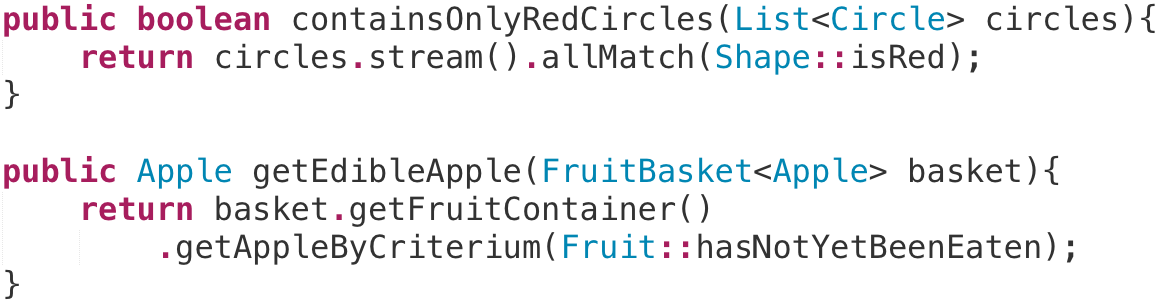
\includegraphics[width=1\columnwidth]{img/type2}
  \caption{Example of a type 2 clone.}
  \label{fig:type2}
\end{figure}

The example in Fig.~\ref{fig:type2} shows a type 2 clone that poses no harm to the design of the system. Both methods are, except for their matching structure, completely different in functionality. They operate on different types, call different methods, return different things, etc. Having such a method flagged as a clone does not provide much useful information.

When looking at refactoring, type 2 clones can be difficult to refactor. For instance, if we have variability in types, the code can describe operations on two completely dissimilar types. Type 2 clones do not differentiate between primitives and reference types, which further undermines the usefulness of clones detected by this definition.

\subsection{Type 3 clones}\label{sec:type3}
Type 3 clones are \textit{copied fragments with further modification (having added, removed or changed statements)}~\cite{roy2007survey}. Detection of clones by this definition can be hard, as it may be hard to detect whether a fragment was copied in the first place if it was severely changed. Because of this, most clone detection implementations of type 3 clones work on basis of a similarity threshold~\cite{roy2008nicad,ragkhitwetsagul2019siamese,jiang2007deckard,semura2017ccfindersw}. This similarity threshold has been implemented in different ways: textual similarity (for instance using Levenshtein distance)~\cite{lavoie2011automated}, token-level similarity~\cite{sajnani2016sourcerercc} or statement-level similarity~\cite{kamalpriya2017enhancing}.

Having a definition that allows for any change in code poses serious challenges on refactoring. A Levenshtein distance of one can already change the meaning of a code fragment significantly, for instance, if the name of a type differs by a character (and thus referring to different types).

\subsection{Refactoring-oriented clone types}\label{sec:rtypes}
To resolve the shortcomings of clone types as outlined in the previous section, we propose alternative definitions for clone types directed at detecting clones that can and should be refactored. We have named these clones T1R (type 1R), T2R and T3R clones. These definitions address problems of the corresponding literature definitions. The ``R'' stands for refactoring-oriented.

\subsubsection{Type 1R clones} \label{sec:type1r}
To solve the issues identified in Sec.~\ref{sec:type1}, we introduce an alternative definition: cloned fragments have to be both textually \textit{and} functionally equal. Therefore, T1R clones are a subset of type 1 clones.
%Although requiring fragments to be functionally equal, T1R clones do not allow for change in implementation (like type 4 clones).

We check functional equality of two fragments by comparing the equality of the fully qualified identifier (FQI) for referenced types, methods and variables. If an identifier is fully qualified, it means we specify the full location of its declaration (e.g. \texttt{com.sb.fruit.Apple} for an \texttt{Apple} object). For method calls, we also compare the equality of the FQI of the type of each of its arguments, to differentiate between overloaded method variants.

\subsubsection{Type 2R clones}\label{sec:type2r}
To solve the issues identifier in Sec.~\ref{sec:type2}, we introduce an alternative definition. All rules that apply to T1R clones also apply to T2R clones. Additionally, T2R clones allow variability in literals, variables and method calls. Furthermore, T2R clones allow variability in method names and class/enum/interface names.

When refactoring two fragments that differ by literals, called methods or used variables, we are faced with a design tradeoff. When replacing the cloned fragments by a new method, we need an extra argument for each literal, called method or used variable that differs. This can be done as long as the type of used literals/variables and the signature of called methods are equal.

To limit the negative impact of this tradeoff on the design of the system, we formalized a threshold for the variability between fragments. The formula by which this threshold is calculated is displayed in equation \ref{eq:type2r}. In this formula, \textit{different expressions} refers to the number of literals, variables and method calls that differ from other clone instances in a clone class. We divide this by the total number of tokens in the clone instance. Based on this threshold, we decide whether a clone should be considered for refactoring.

\begin{equation}\label{eq:type2r}
\text{T2R Variability}=\frac{\text{Different expressions}}{\text{Total tokens}}*100
\end{equation}

\subsubsection{Type 3R clones}\label{sec:type3r}
Type 3 clones allow any change in statements (added, removed and changed statements). When looking at how we can refactor a statement that is not included by one clone instance but is in another, we find that we require a conditional block to make up for the difference in statements. This is a tradeoff, as an added conditional block increases the complexity of the system. Because of that, we defined T3R clones in such a way that they are directed towards finding clones that are worth this tradeoff.

All rules that apply to T2R clones also apply to T3R clones. Additionally, T3R clones allow a gap between two clone classes of statements that are not cloned. The following rules apply to this gap:

\begin{itemize}
  \item \textbf{The difference in statements must bridge a gap between two clones that were valid by the original thresholds}. This entails that, different from type 3 clones, the difference in statements cannot be at the beginning or the end of a cloned block. It is rather somewhere within, as it must bridge two existent clones.
  \item \textbf{The size of the gap between two clones is limited by a threshold.} This threshold is calculated by taking the percentage of the number of statements in the gap over the number of statements that both clones that are being bridged span. This is displayed in equation \ref{eq:type3r}.
  \item \textbf{The gap may not span a partial block.} To make sure that the T3R clone can be refactored, we do not allow the gap to span a part of a block, for instance, the declaration and a part of the body of a for-loop. The reason for this is that it is not possible to wrap a partially spanned block in a single conditional statement. We could, however, use multiple conditional blocks (one for each block spanned), but due to the detrimental effect on the design of the code (as each conditional block adds a certain complexity), we decided not to allow this for T3R clones.
\end{itemize}

\begin{equation}\label{eq:type3r}
\text{T3R Gap Size}=\frac{\text{Statements in gap}}{\text{Statements in clones}}*100
\end{equation}

\subsubsection{The challenge of detecting these clones}\label{chap:challenge}
To detect each type of clone, we need to parse the FQI of all types, method calls, and variables. This comes with challenges, regarding both performance and implementation. To trace the declarations of variables, methods, and types, we might need to follow cross-file references. The referenced types/variables/methods might even not be part of the project, but rather of an external library or the standard libraries of the programming language. All these factors need to be considered for the referenced entity to be found, on basis of which an FQI can be created.

\section{Clone Detection}\label{chap:clonedetection}
As duplication in source code is a serious problem in many software systems, many tools have been proposed to detect various types of code clones~\cite{sheneamer2016survey, svajlenko2014evaluating}. However, these tools were not yet assessed in terms of automatically refactoring clones. In this section, we first assess a set of modern clone detection tools for their applicability to this domain. Next, we introduce our own tool geared towards automatic clone refactoring, CloneRefactor.%Two surveys of modern clone detection tools~\cite{sheneamer2016survey, svajlenko2014evaluating} together show an overview of the most-popular clone detection tools up until 2016. \todo{what is insufficient about these two? what triggered the need to reassess clone detectors? where are the four criteria coming from?}

\subsection{Survey on Clone Detection Tools}
\label{ch:tool-overview}
We conducted a short survey on (recent) clone detection tools that we could use to analyze refactoring possibilities. The results of our survey are displayed in table~\ref{table:dettools}. We chose a set of tools that are open source and can analyze a popular object-oriented programming language. Next, we formulate the following four criteria by which we analyze these tools:
\begin{enumerate}
    \item \textbf{Should find clones in any context.} Some tools only find clones in specific contexts, such as only method level clones. We want to perform an analysis of all clones in projects to get a complete overview.
\item \textbf{Finds clone classes in control projects.} We assembled a number of control projects to assess the validity of clone detection tools.
\item \textbf{Can analyze resolved symbols.} When detecting the types proposed in section \ref{sec:rtypes}, it is important that we can analyze FQIs of symbols. The rationale for this is further explained in \ref{chap:challenge}.
\item \textbf{Extensive detection configuration.} We aim to exclude expressions/statements from matching (more about our rationale in section~\ref{sec:rtypes}). To achieve this, the tool needs to be able to allow those threshold changes. This can be either through simple changes of the source code or by using some configuration file.
\end{enumerate}

\begin{table}[H]
 \begin{center}
  \caption{Our survey on clone detection tools.} \label{table:dettools}
  \medskip
\begin{tabular}{|l|l|l|l|l|l|}
\hline
\textbf{Clone Detection Tool} & \textbf{(1)} & \textbf{(2)} & \textbf{(3)} & \textbf{(4)} \\ \hline
Siamese~\cite{ragkhitwetsagul2019siamese} &  &             &             & \checkmark            \\ \hline
NiCAD~\cite{roy2008nicad, cordy2011nicad} & \checkmark                             & \checkmark            &             &             \\ \hline
CPD~\cite{roy2009comparison} & \checkmark & \checkmark            &             &             \\ \hline
\begin{tabular}[c]{@{}l@{}}CCFinder~\cite{kamiya2002ccfinder}\\ D-CCFinder~\cite{livieri2007very}\end{tabular} & \checkmark  & \checkmark   &    &   \\ \hline
CCFinderSW~\cite{semura2017ccfindersw}   & \checkmark     &             &             & \checkmark            \\ \hline
\begin{tabular}[c]{@{}l@{}}SourcererCC~\cite{sajnani2016sourcerercc}\\ Oreo~\cite{saini2018oreo}\end{tabular} & \checkmark    &             &             & \checkmark            \\ \hline
BigCloneEval~\cite{svajlenko2016bigcloneeval}  & \checkmark  & \checkmark   &             &             \\ \hline
Deckard~\cite{jiang2007deckard} & \checkmark   &             & \checkmark            &             \\ \hline
Scorpio~\cite{higo2013revisiting, kamalpriya2017enhancing} & \checkmark   &     & \checkmark  & \checkmark   \\ \hline
\end{tabular}
\end{center}
\end{table}

Apart from these criteria, we found that the output of these clone detection tools cannot be post-processed to find the clone types proposed in section \ref{sec:rtypes}. This is mainly because the clones of T2R are not a subset of type 2 clones and will thus require an analysis of the entire system.

\subsection{CloneRefactor}
None of the state-of-the-art tools we identified implement all our criteria, so we decided to implement our own clone detection tool: CloneRefactor\footnote{CloneRefactor (WIP) is available on GitHub: \url{https://github.com/SimonBaars/CloneRefactor}}. In this tool, we implemented both the literature clone types~\cite{roy2007survey} and our refactoring-oriented clone types as described in Sec.~\ref{sec:rtypes}. %An abstract view of the process flow of CloneRefactor is displayed in figure \ref{fig:clonerefactor}

%\begin{figure}[H]
%  \caption{Abstract representation of CloneRefactor.}
%    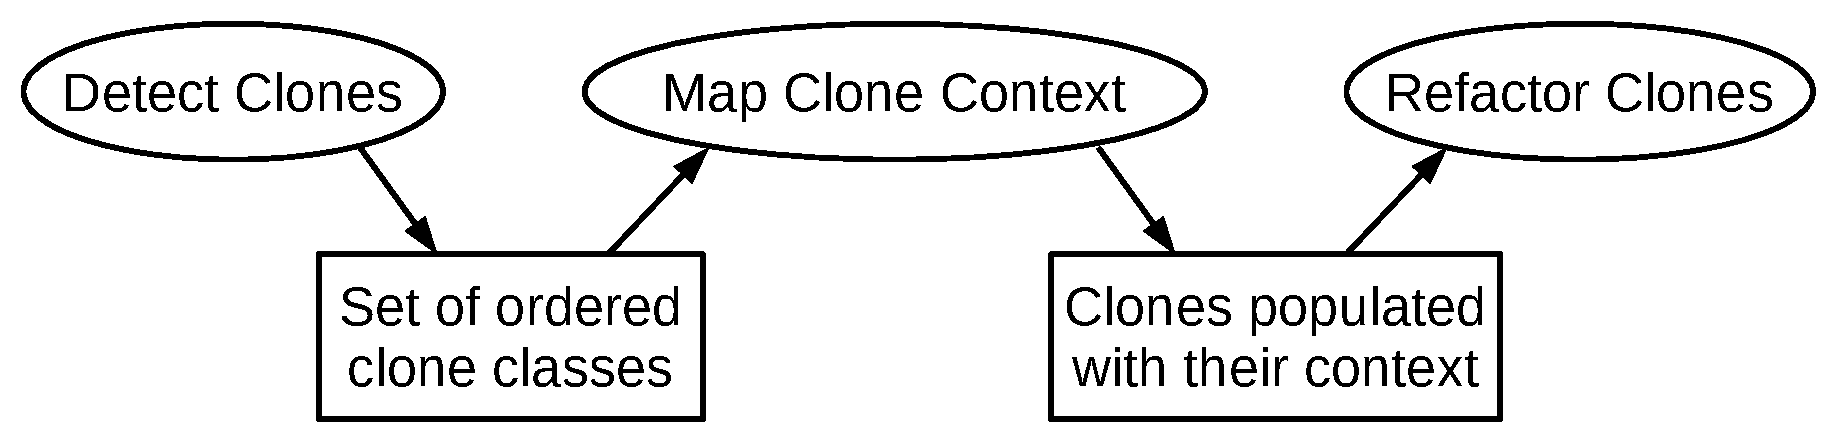
\includegraphics[width=1\columnwidth]{img/CloneRefactorOverall}
%  \label{fig:clonerefactor}
%\end{figure}

Our tool is based on the JavaParser library~\cite{tomassetti2017javaparser}. This library can parse Java source code to an AST representation. This AST can then be analyzed, modified and eventually written back to source code. This allows us to perform AST-based clone detection and apply transformations to the AST based on the clones found.

CloneRefactor walks the AST and collects each declaration and statement (similar to the Scorpio clone detection tool~\cite{higo2013revisiting}). It then builds a graph representation on basis of this AST, in which each declaration and statement becomes a node. This graph representation maps the following relations for each declaration and statement:

\begin{itemize}
  \item The declaration/statement preceding it
  \item The declaration/statement following it
  \item The previous statement/declaration that is cloned
\end{itemize}

Whether a node is considered a clone depends on the clone type that is being analyzed. On basis of this graph, we detect clone classes. We compare clone classes against thresholds and remove the clone classes that do not pass the test.

\section{Experiments}
This section outlines the conducted experiments to determine refactoring opportunities for code clones. We show the corpus on which we have performed our measurements in section \ref{chap:corpus}. Next, we look into the thresholds that determine whether duplicated fragments are considered a clone in section \ref{chap:thresholds}. We then show a comparison between the different proposed clone types in section \ref{sec:clonetypeexperiments}. Afterward, we perform an analysis of the context of code clones in section \ref{chap:clonecontextexpl}. Finally, we map refactoring opportunities for clones in section \ref{chap:mergingdups}.

All experiments were conducted using CloneRefactor, which contains scripts for running large scale clone detection over the indicated corpus.

\subsection{The corpus}\label{chap:corpus}
For our experiments, we use a large corpus of open source projects~\cite{githubCorpus2013}. This corpus has been assembled to contain relatively higher quality projects. Also, any duplicate projects and files were removed from this corpus. This results in a variety of Java projects that reflect the quality of average open source Java systems and are useful to perform measurements on. We filtered this corpus further to only include projects that use Maven, which is a build tool which is mainly used to manage dependencies in the Java ecosystem. We then filtered the corpus further to only include projects for which all external dependencies are available, as CloneRefactor requires all dependencies of a project in order to accurately resolve all its symbols. This resulted in 1.343 projects of varying sizes averaging at 980 source lines of code (omitting whitespace, comments) per project.

\subsection{Thresholds}\label{chap:thresholds}
Thresholds are a tool that aid in the process of deciding whether a clone \textit{should} be refactored. Many clone detection tools focus on either the number of lines~\cite{kamiya2002ccfinder, svajlenko2016bigcloneeval}, number of tokens~\cite{roy2008nicad, sajnani2016sourcerercc, ragkhitwetsagul2019siamese} and/or number of nodes (declarations/statements)~\cite{higo2013revisiting} to decide whether code fragments should be considered clones of each other. A comparison of clone detection tools by Bellon et al.~\cite{bellon2007comparison} shows that most clone detection tools choose a minimum of \textbf{6} lines of code to be duplicate to consider code fragments a clone. The Scorpio clone detection tool uses this same number as minimum the number of nodes~\cite{higo2013revisiting}. Many token based tools use a threshold of \textbf{50} tokens for fragments to be considered a clone~\cite{sajnani2016sourcerercc}.

We would argue that going with this ``magic number 6'' eliminates a lot of harmful clones that should be refactored. For instance, a single 100-token statement will not be considered by such a threshold, which can still be harmful to the system design when cloned. Because of that, we decided to perform our measurements using thresholds that will include most clones that should be refactored, while eliminating most of the noise. With ``noise'' we mean duplication that has no relevancy towards refactoring, like a single token that is duplicated elsewhere.

To find such a threshold, we measured the number of clone classes found for a certain number of tokens. We then looked at the number of nodes (statements/declarations) that these clones span. The resulting chart is displayed in Fig.~\ref{fig:tokenthreshold}.

\begin{figure}[H]
  \caption{Amount of times a clone with a certain number of tokens has a certain number of nodes.}
    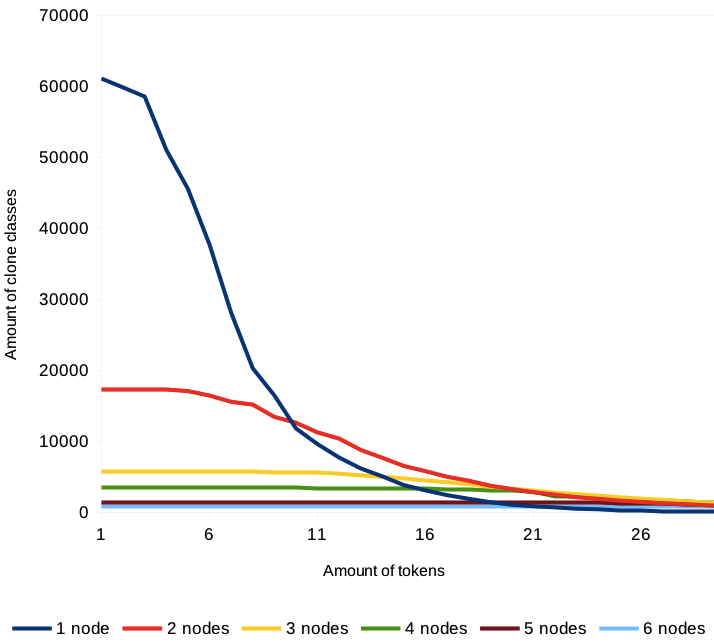
\includegraphics[width=.95\columnwidth]{img/TokenThreshold}
  \label{fig:tokenthreshold}
\end{figure}

In this chart, we see that when seeking clones with a minimum of 10 tokens, there are more clones that span 2 statements than clones that span one statement. We manually assessed these clones, and mainly the two-statement clones contain many clones that we classified as ``should be refactored''. Because of this, we decided to go with a minimum of 10 tokens threshold for our experiments.

\subsection{Clone types}\label{sec:clonetypeexperiments}
In this chapter we display the differences between clone type 1-3~\cite{roy2007survey} and type 1R-3R as proposed in section \ref{sec:rtypes}. When running our clone detection script over the corpus, we get the results displayed in Fig.~\ref{fig:typeres}.

\begin{figure}[H]
  \caption{Number of cloned declarations/statements.}
    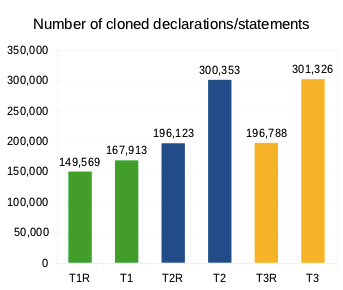
\includegraphics[width=.9\columnwidth]{img/TypeResults}
  \label{fig:typeres}
\end{figure}

In this figure, the number of cloned nodes per clone type are displayed. The difference between T1R and T1 is small (10.9\%), because most often textually equal code is also functionally equal. The difference between T2R and T2 is bigger (34.7\%) because the T2R definition is more strict. T3R and T3 are similar to T2R and T2 because our dataset does not have so many gapped clones for the thresholds used.

We also measured the duration of finding clones by the different clone types. Fig.~\ref{fig:performance} shows the duration of detecting all clones in the corpus using CloneRefactor for different clone types. Although this data is partly dependent on our implementation of the clone types, there is a notable difference between the refactoring-oriented clone types and the literature clone types. The reason for this is further explained in section \ref{chap:challenge}.

\begin{figure}[H]
  \caption{Duration in minutes of identifying clones for clone type definitions.}
    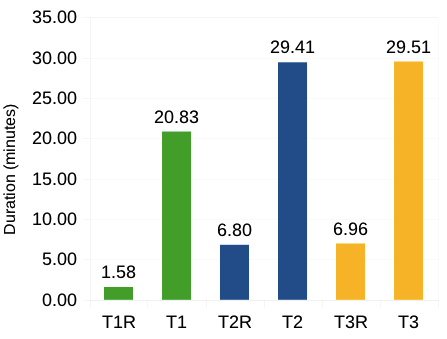
\includegraphics[width=.9\columnwidth]{img/DurationChart}
  \label{fig:performance}
\end{figure}

\subsection{Context Analysis of Clones}\label{chap:clonecontextexpl}
To be able to refactor code clones, it is important to consider the context of the clone. We define the following aspects of the clone as its context:
\begin{enumerate}
  \item \textbf{Relation:} The relation of clone instances among each other through inheritance.
  \item \textbf{Location:} Where a clone instance occurs in the code.
  \item \textbf{Contents:} The statements/declarations of a clone instance.
\end{enumerate}
We perform experiments on each of these aspects, defining categories and measuring these categories over the corpus.

\begin{figure}[H]
  \caption{Abstract representation of clone classes and clone instances.}
    \medskip
    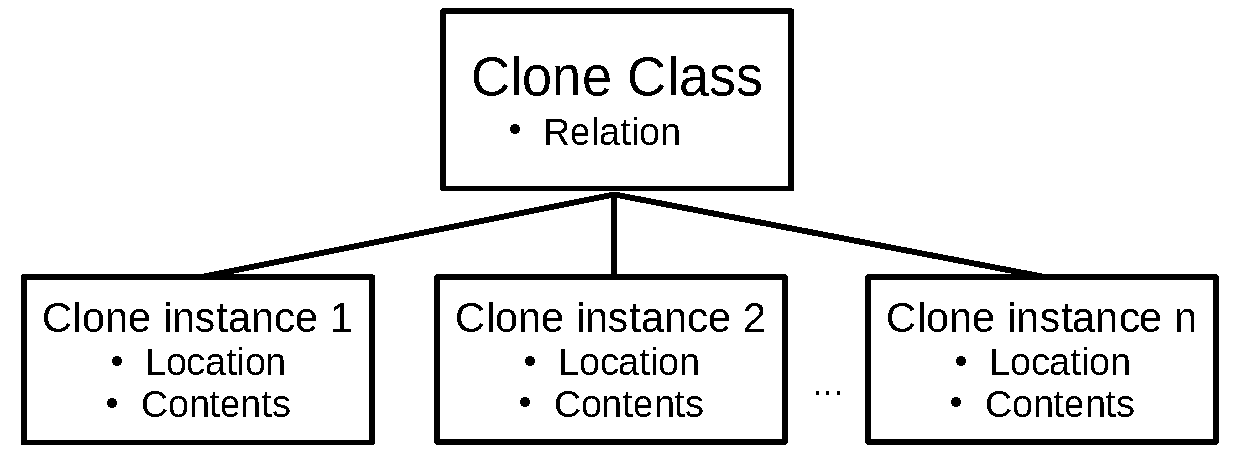
\includegraphics[width=1\columnwidth]{img/context}
  \label{fig:clonecontext}
\end{figure}

Fig.~\ref{fig:clonecontext} shows an abstract representation of clone classes and clone instances. The relation of clones through inheritance is measured for each clone class. The location and contents of clones are measured for each clone instance.

All data shown in this section is measured using the T1R clone definition. We have performed the same measurements for the other type definitions and found that they follow similar trends. Because of that, we decided not to further show them in this section.

\subsubsection{Relations Between Clone Instances} \label{chap:relationsinstances}
When merging code clones in object-oriented languages, it is important to consider the inheritance relation between clone instances. This relation has a big impact on how a clone should be refactored.

Fontana et al.~\cite{fontana2015duplicated} describe measurements on 50 open source projects on the relation of clone instances to each other. To do this, they first define several categories for the relation between clone instances in object-oriented languages. These categories are as follows:
\begin{enumerate}
  \item \textbf{Same method}: All instances of the clone class are in the same method.
  \item \textbf{Same class}: All instances of the clone class are in the same class.
  \item \textbf{Superclass}: All instances of the clone class are child or parent of each other.
  \item \textbf{Ancestor class}: All instances of the clone class are superclasses except for the direct superclass.
  \item \textbf{Sibling class}: All instances of the clone class have the same parent class.
  \item \textbf{First cousin class}: All instances of the clone class have the same grandparent class.
\item \textbf{Common hierarchy class}: All instances of the clone class belong to the same inheritance hierarchy, but do not belong to any of the other categories.
\item \textbf{Same external superclass}: All instances of the clone class have the same superclass, but this superclass is not included in the project but part of a library.
\item \textbf{Unrelated class}: There is at least one instance in the clone class that is not in the same hierarchy.
\end{enumerate}

\begin{figure}[H]
  \caption{Abstract figure displaying relations of clone classes. Arrows represent superclass relations.}
    \medskip
    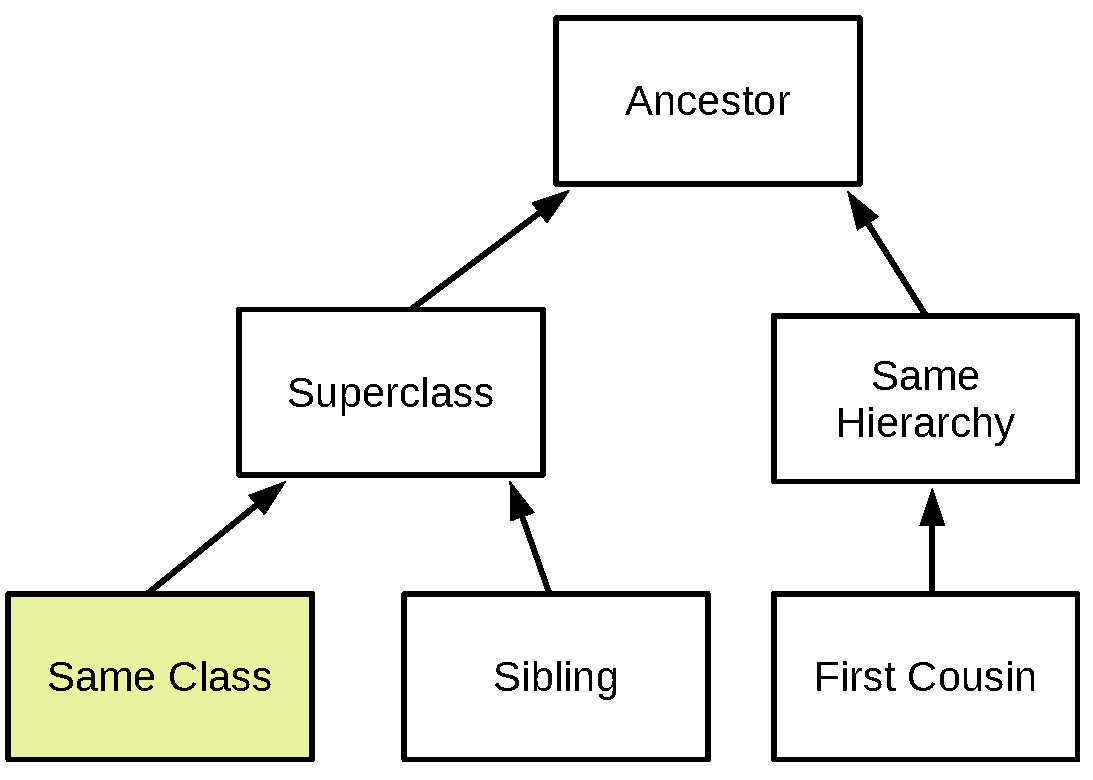
\includegraphics[width=1\columnwidth]{img/Relation}
  \label{fig:clonerelation}
\end{figure}

We use a similar setup to that used by Fontana et al. (Table~3 of Fontana et al.~\cite{fontana2015duplicated}). Fontana et al. measure clones using their own tool (DCRA). As explained in section~\ref{ch:tool-overview}, we chose to implement our own tool, CloneRefactor. Therefore, the setup for our measurements differs as follows from Fontana et al.:
\begin{itemize}
  \item We consider clone classes rather than clone pairs. The rationale for this is given in Sec.~\ref{chap:cloneclasses}.
\item We use different thresholds regarding when a clone should be considered. Fontana et al. seek clones that span a minimum of 7 source lines of code (SLOC). We seek clones with a minimum size of 6 statements/declarations. This is explained detail in Sec.~\ref{chap:thresholds}.
\item We seek duplicates by statement/declaration rather than SLOC. This makes our analysis depend less on the coding style (in terms of newline usage) of the author of the software project.
\item We test a broader range of projects. Fontana et al. use a set of 50 relatively large projects. We use the corpus as explained in \ref{chap:corpus}, which contains a diverse set of projects (diverse both in volume and code quality).
\end{itemize}

Table~\ref{table:relations} contains our results regarding the relations between clone instances.

\begin{table}[H]
  \begin{center}
  \caption{Clone relations} \label{table:relations}
  \medskip
\begin{tabular}{|l|l|l|} \hline
\textbf{Relation} & \textbf{\#} & \textbf{\%} \\ \hline
Unrelated          & 12,368 & 34.88            \\ \hline
Same Class          & 11,483 & 32.38             \\ \hline
Same Method               & 5,056 & 14.26            \\ \hline
Sibling         & 4,182 & 11.79             \\ \hline
External Superclass   & 1,066 & 3.01             \\ \hline
Superclass          & 558 & 1.57           \\ \hline
First Cousin          & 489 & 1.38           \\ \hline
Common Hierarchy    & 206 & 0.58            \\ \hline
Ancestor          & 54 & 0.15          \\ \hline
\end{tabular}
\end{center}
\end{table}

The most notable difference when comparing it to the results of Fontana et al.~\cite{fontana2015duplicated} is that in our results most of the clones are unrelated (34.44\%), while for them it was only 15.70\%. This is likely due to the fact that we consider clone classes rather than clone pairs, and mark the clone class ``Unrelated'' even if just one of the clone instances is outside a hierarchy. It could also be that the corpus which we use, as it has generally smaller projects, uses more classes from outside the project (which are marked ``Unrelated'' if they do not have a common external superclass). About a third of all clone classes have all instances in the same class, which is generally easy to refactor. On the third place come the clones that are in the same method, which are similarly easy to refactor.

\subsubsection{Clone instance location}\label{chap:clonelocation}
After mapping the relations between individual clones, we considered at the location of individual clone instances. A paper by Lozano et al.~\cite{lozano2007evaluating} discusses the harmfulness of cloning. The authors argue that 98\% are produced at method level. However, this claim is based on a small dataset and based on human copy-paste behavior rather than static code analysis. We validated this claim over our corpus, using the following categories:
\begin{enumerate}
  \item \textbf{Method/Constructor Level:} A clone instance that does not exceed the boundaries of a single method or constructor (optionally including the declaration of the method or constructor itself).
  \item \textbf{Class Level:} A clone instance in a class, that exceeds the boundaries of a single method or contains something else in the class (like field declarations, other methods, etc.).
  \item \textbf{Interface/Enumeration Level:} A clone that is (a part of) an interface or enumeration.
\end{enumerate}

The results are shown in Table~\ref{table:locations}. Our results indicate that, quite significantly, most clones are found at methodlevel. The number of clones found in interfaces and enumerations is very low.

\begin{table}[H]
  \begin{center}
  \caption{Clone instance locations} \label{table:locations}
  \medskip
\begin{tabular}{|l|l|l|}
\hline
\textbf{Location}   & \textbf{\#} & \textbf{\%} \\ \hline
Method Level        & 83,813 & 82.62            \\ \hline
Class Level        & 12,534 & 12.35            \\ \hline
Constructor Level    & 4,391 & 4.33           \\ \hline
Interface Level   & 567 & 0.56           \\ \hline
Enum Level         & 145 & 0.14            \\ \hline
\end{tabular}
\end{center}
\end{table}

\subsubsection{Clone instance contents}\label{chap:clonecontents}
Finally, we looked at the contents of individual clone instances: what combination of declarations and statements they span. We selected the following categories to be relevant for refactoring:
\begin{enumerate}
  \item \textbf{Full Method/Class/Interface/Enumeration:} A clone that spans a full class, method, constructor, interface or enumeration, including its declaration.
  \item \textbf{Partial Method/Constructor:} A clone that spans a method partially.
  \item \textbf{Several Methods:} A clone that spans over two or more methods, either fully or partially.
  \item \textbf{Only Fields:} A clone that spans only global variables.
  \item \textbf{Includes Fields/Constructor:} A clone that spans fields/constructors, but can also span other statements or declarations.
  \item \textbf{Method/Class/Interface/Enumeration Declaration:} A clone that contains the declaration (usually the first line) of a class, method, interface or enumeration.
\end{enumerate}

The results for these categories are displayed in Table \ref{table:contents}.

\begin{table}[H]
  \begin{center}
  \caption{Clone instance contents} \label{table:contents}
  \medskip
\begin{tabular}{|l|l|l|}
  \hline
  \textbf{Contents} & \textbf{\#} & \textbf{\%} \\ \hline
  Partial Method     & 79,945 & 78.80 \\ \hline
  Several Methods         & 7,323 & 7.22 \\ \hline
  Partial Constructor      & 4,385 & 4.32 \\ \hline
  Full Method           & 3,868 & 3.81 \\ \hline
  Only Fields           & 3,039 & 3.00 \\ \hline
  Includes Constructor  & 1,522 & 1.50 \\ \hline
  Includes Field        & 616 & 0.61 \\ \hline
  Includes Class Declaration  & 376 & 0.37 \\ \hline
  Other Categories    & 376 & 0.37\\ \hline
\end{tabular}
\end{center}
\end{table}

Unsurprisingly, most clones span a part of a method. The most used refactoring technique for clones that span part of a method is ``Extract Method''. Because of that, we focus our research efforts on refactoring such clones.

\subsection{Method extraction opportunities}\label{chap:mergingdups}
The most used technique to refactor clones is method extraction (creating a new method on basis of the contents of clones). However, method extraction cannot be applied in all cases. In these instances, more conditions may apply to be able to conduct a refactoring, if beneficial at all.

We measured the number of clones that can be refactored through method extraction (without additional transformations being required). Our results are displayed in Table \ref{table:refactorability}. In this table we use the following categories:
\begin{itemize}
    \item \textbf{Can be extracted:} This clone is a fragment of code that can directly be extracted to a method. Then, based on the relation between the clone instances, further refactoring techniques can be used to refactor the extracted methods (for instance ``pull up method'' for clones in sibling classes).
    \item \textbf{Complex control flow:} This clone contains \texttt{break}, \texttt{continue} or \texttt{return} statements, obstructing the possibility of method extraction.
    \item \textbf{Spans part of a block:} This clone spans a part of a statement.
    \item \textbf{Is not a partial method:} If the clone does not fall in the ``Partial method'' category of Table \ref{table:contents}, the ``extract method'' refactoring technique cannot be applied.
\end{itemize}

\begin{table}[H]
  \begin{center}
  \caption{Refactorability through method extraction} \label{table:refactorability}
  \medskip
\begin{tabular}{|l|l|l|}
\hline
\textbf{}         & \textbf{\#} & \textbf{\%} \\ \hline
Can be extracted     & 13,553 & 38.22 \\ \hline
Spans part of a block  & 12,332 & 34.78 \\ \hline
Is not a partial method   & 8,074 & 22.77 \\ \hline
Complex control flow & 1,503 & 4.24 \\ \hline
\end{tabular}
\end{center}
\end{table}

From Table \ref{table:refactorability}, we can see that 38.22\% of the clones can directly be refactored through method extraction (and possibly other refactoring techniques based on the relation of the clone instances). For the other clones, other techniques or transformations will be required.

\section{Threats to validity}\label{chap:threatstovalidity}
We noticed that, when doing measurements on a corpus of this size, the thresholds that we use for the clone detection have a big impact on the results. There does not seem to be one golden set of thresholds, some thresholds work in some situations but fail in others. We have chosen thresholds that, according to our experiments and assessments, seemed optimal. However, by using these, we might have some ``noise'' in our results of clones that should not be considered for refactoring.

\section{Conclusion and next steps}\label{chap:conclusion}
In the research we have conducted so far we have made three novel contributions:
\begin{itemize}
    \item We proposed a method with which we can detect clones that can/should be refactored.
    \item We mapped the context of clones in a large corpus of open source systems.
    \item We mapped the opportunities to perform method extraction on clones this corpus.
\end{itemize}

We have looked into existing definitions for different types of clones~\cite{roy2007survey} and proposed solutions for problems that these types have with regards to automated refactoring. We propose that fully qualified identifiers (FQIs) of method call signatures and type references should be considered instead of their plain text representation, to ensure refactorability. Furthermore, we propose that one should define a threshold for variability in variables, literals, and method calls, in order to limit the number of parameters that the refactored method will have.

The research that we have conducted so far analyzes the context of different kinds of clones and prioritizes their refactoring. Firstly, we looked at the inheritance relation of clone instances in a clone class. We have found that a little more than a third of all clone classes are flagged unrelated, which means that they have at least one instance that has no relation through inheritance with the other instances. About a third of the clone classes all of its instances are in the same class.

Secondly, we looked at the location of clone instances. Most clone instances (79 percent) are found at method level. Because of that, we concluded that our main refactoring focus should be aimed at method level clones. A common method to refactor such clones is by extracting a new method on basis of the contents of the clone. However, method extraction cannot be applied in all cases. According to our experiments, about 40 percent of the clones can be refactored by extracting them to a new method.

\subsection{Next steps}
Our next step is to implement the ``Extract Method'' refactoring for the identified automatic refactoring opportunities. On basis of the resulting code, we can perform experiments that compare the maintainability index of the refactored code to the original code. The maintainability index of a system is an aggregation of various metrics that test a systems' maintainability (like volume, complexity, duplication, etc.). If we can automatically apply refactorings to the identified clones, this maintainability index can be used to select more optimal threshold values.

\section*{Acknowledgements}
We would like to thank the Software Improvement Group (SIG) for their continuous support in this project.

\bibliographystyle{alpha}
\bibliography{res}

\end{document}
